\documentclass[12pt,twoside,a4paper,tikz,border=5]{refart} 
% add russian language
\usepackage[utf8]{inputenc}
\usepackage[T1]{fontenc}
\usepackage[russian]{babel}
% make the first line of all sections be indented by the usual paragraph indentation
\usepackage{indentfirst}
\setlength{\parindent}{1cm} % paragraph indent

% for no sign
\usepackage{textcomp}
% for tikz
\usepackage{pgf,tikz}
\usepackage{mathrsfs}
\usetikzlibrary{arrows}

% for table columns

\usepackage{array}
%\newcolumntype{L}[1]{>{\raggedright\let\newline\\\arraybackslash\hspace{0pt}}m{#1}}
%\newcolumntype{C}[1]{>{\centering\let\newline\\\arraybackslash\hspace{0pt}}m{#1}}
%\newcolumntype{R}[1]{>{\raggedleft\let\newline\\\arraybackslash\hspace{0pt}}m{#1}}

\newcolumntype{Z}{>{\centering\let\newline\\\arraybackslash\hspace{0pt}}X} 
\newcolumntype{M}{>{\raggedright\let\newline\\\arraybackslash\hspace{0pt}}X}
\newcolumntype{L}[1]{>{\raggedright\let\newline\\\arraybackslash\hspace{0pt}}m{#1}}
\newcolumntype{C}[1]{>{\centering\let\newline\\\arraybackslash\hspace{0pt}}m{#1}}


% for code listings
\usepackage{listings}
\usepackage{color}

\definecolor{codegreen}{rgb}{0,0.6,0}
\definecolor{codegray}{rgb}{0.5,0.5,0.5}
\definecolor{codepurple}{rgb}{0.58,0,0.82}
\definecolor{backcolour}{rgb}{0.95,0.95,0.92}

\lstdefinestyle{mystyle}{
	backgroundcolor=\color{backcolour},   
	commentstyle=\color{codegreen},
	keywordstyle=\color{magenta},
	numberstyle=\color{codegray},
	stringstyle=\color{codepurple},
	basicstyle=\linespread{1}\footnotesize\ttfamily,
	breakatwhitespace=false,         
	breaklines=true,                 
	captionpos=b,                    
	keepspaces=true,                 
	numbers=left,                    
	numbersep=5pt,                  
	showspaces=false,                
	showstringspaces=false,
	showtabs=false,                  
	tabsize=2,
}

\lstset{style=mystyle}

% for empty set
\usepackage{amssymb}
%brackets for equation refs
\usepackage{amsmath}
% line interval
\usepackage{setspace}
\setstretch{1.5}


% setup titles 
\usepackage{titlesec}
	\titleformat{\section}
		{\normalfont\fontsize{16}{0}\bfseries}{\thesection}{1em}{}
	\titleformat{\subsection}
		{\normalfont\fontsize{14}{0}\bfseries}{\thesubsection}{1em}{}
	\titleformat{\subsubsection}
		{\bf\fontsize{14}{0}}{\thesubsubsection}{1em}{}

	\titlespacing*{\section}
		{0pt}{5ex}{3ex} % left before after
	\titlespacing*{\subsection}
		{0pt}{3ex}{1ex}
	\titlespacing*{\subsubsection}
		{0pt}{3ex}{1ex}
	%start each section on new page
	\newcommand{\sectionbreak}{\clearpage}


% set up better resolution
\pdfpkmode{dpdfezzz}
\pdfpkresolution=8000

% set fraction of text
\settextfraction{0.88}

%colorbox for menu
\usepackage[most]{tcolorbox}
\definecolor{myblue}{rgb}{0.000, 1.000, 1.000}
\definecolor{dodgerblue}{rgb}{0.117,0.564,1.000}


\newtcolorbox[auto counter]{guide}[1][]{enhanced jigsaw,inherit height,
	colback=red!5,opacityback=0.9,colframe=red,title=Алгоритм \#\thetcbcounter,
	grow to left by=4mm,grow to right by=4mm,
	arc is angular,arc=0mm,
	fonttitle=\bfseries\large,
}

\newtcbtheorem[auto counter]{algorithm}{Алгоритм}{
	breakable,
	lower separated=false,
	colback=white!80!gray,
	colframe=white, fonttitle=\bfseries,
	colbacktitle=white!50!gray,
	coltitle=black,
	enhanced,
	boxed title style={colframe=black},
	after skip=20pt
}{alg}


% for figures
\usepackage{subcaption}
\DeclareCaptionLabelFormat{gostfigure}{Рисунок #2}
\DeclareCaptionLabelFormat{slide}{Слайд №#2}
\DeclareCaptionLabelFormat{gosttable}{Таблица #2}
\DeclareCaptionLabelSeparator{gost}{~---~}

\captionsetup{labelsep=gost}
\captionsetup[figure]{labelformat=gostfigure}
\captionsetup[table]{labelformat=gosttable}
\captionsetup{figurewithin=none, tablewithin=none}
\renewcommand{\thesubfigure}{\asbuk{subfigure}}

%for crop
\usepackage{graphicx}
\usepackage{grffile}

% for tables and image inside
\usepackage{array}
\usepackage{tabularx,booktabs} 
% biblio style
\bibliographystyle{utf8gost705u} 

% for margins
\setlength\oddsidemargin{-0in}
\setlength\evensidemargin{-0in}
\setlength\textwidth{165mm}

% for web links
\usepackage{hyperref}
\hypersetup{
	colorlinks=true,
	linkcolor=blue,
	urlcolor=blue,
}

\urlstyle{same}

% for header on every page
\usepackage{fancyhdr}
\usepackage{lipsum}% just to generate text for the example

\pagestyle{fancy}
\fancyhf{}
\fancyhead[L]{\rightmark}
\fancyhead[R]{\thepage}
\renewcommand{\headrulewidth}{0.4pt}
%\renewcommand{\footrulewidth}{0.4pt}% default is 0pt

% Tables and pictures captions align
\usepackage[]{caption}
\captionsetup[table]{justification=raggedleft} 
\captionsetup[figure]{justification=centering,labelsep=endash} 

% for enumerate style
\renewcommand\labelenumii{\theenumi.\arabic{enumii}.}

% for pagebreak in tabularx
\usepackage{tabularx}
\usepackage{tabu}

\newcounter{titem}[table]
\newenvironment{titem}[2][]{\refstepcounter{titem}\par\medskip
	\noindent \textit{
		\begin{flushleft}
			\begin{hyphenrules}{nohyphenation}
				\thetitem.~#1~#2\newline
			\end{hyphenrules}
		\end{flushleft}
	}}{\medskip}

\begin{document}
	\begin{titlepage}
		\centering
		{\scshape\small Национальный исследовательский университет \\
			``Высшая школа экономики'' \par}
		\vspace{2cm}
		{\Huge\bfseries ОТЧЁТ ПО ПРАКТИКЕ\par}
		\vspace{2cm}
		{\scshape\Large Исследование возможного сокращения перебора при выборе параметров $ p, \beta $ \\
			для алгоритма $ A-Ward_{p\beta}$ \par}
		\vspace{1.5cm}
				
		\vfill
		\begin{center}
			\begin{tabular}{  p{7cm}  p{4cm} p{5cm}  } 
				& & \textbf{Студент:}\\ 
				& & Еремейкин П.А. \\ 
				& & группа \\
				& & мНоД16\_ТМСС\\
				& & \\
				& & \textbf{Руководитель: }\\
				& & профессор\\
				& & Миркин Б.Г.\\
			\end{tabular}
		\end{center}
		\vfill
		{Москва \the\year\par}
	\end{titlepage}


	\tableofcontents 
	\newpage
	\section{Основные положения}
		Исследование выполняется в рамках развития пакета программ СИК (Система Интеллектуальной Кластеризации), который был разработан в ходе курсового проекта ``Алгоритмы интеллектуализации метода k-средних''. Этот пакет предназначен для применения современных интеллектуальных методов при решении задач кластеризации. 
		
		В состав пакета входят методы иерархического кластер-анализа: метод аномальных кластеров \cite{anomal-clustering}, алгоритмы $ A-Ward $ , $ A-Ward_{p\beta} $ \cite{a-ward-pb} а также дивизивные методы \cite{kovaleva}. 
		
		С технической точки зрения СИК представляет собой набор Python модулей, объединённых в единую программу при помощи графического пользовательского интерфейса.  
		
		В рамках данной практики рассматривается проблема выбора параметров для алгоритма $ A-Ward_{p\beta} $. Этот алгоритм представляет собой модифицированную версию иерархического алгоритма $ A-Ward $ и вводит два параметра: $ p $ и $ \beta $. Оптимальные значения параметров зависят от конкретной задачи и данных, к которым применяется алгоритм. На настоящее время не существует рекомендаций по эффективному выбору этих параметров, а единственный обоснованный метод --- перебор всех возможных значений с последующей оценкой результата для каждой пары $ (p_i,\beta_i) $  по эмпирической характеристике. Такой подход требует большого времени вычисления, что во многих случаях делает его неприменимым на практике.
		
		Для решения задачи выбора параметров $ p$, $\beta $ в условиях ограниченного времени была выдвинута гипотеза о возможном сокращении перебора. Согласно этой гипотезе, результаты выбора оптимальных значений по всем доступным объектам и по сокращённой выборке из этих объектов различаются не существенно. Цель данной работы состоит в экспериментальной проверке приведённой гипотезы, оценке различных стратегий формирования сокращённой выборки, их характеристик относительно качества результата и затрачиваемого времени.
	
	\section{Алгоритм $ A-Ward_{p\beta} $}
		\subsection{Кластеризация}
			Алгоритм $ A-Ward_{p\beta} $ предназначен для решения задачи кластеризации, то есть выделения из таблиц наблюдения множеств (кластеров) таким образом, чтобы сходные объекты попадали в один и тот же кластер, а несходные --- в разные кластеры \cite{mirkin-ds}. При этом под кластером понимают относительно однородное подмножество объектов, которые характеризуются определёнными признаками. Это подмножество обособлено от остальных объектов.
			
			Задача кластеризации актуальна во многих областях: биологии, социологии, обработке изображений и т.д.
			В качестве примера можно привести задачу выделения таксономических групп из некоторого множества живых организмов, обладающих фиксированными характеристиками, записанными в форме таблицы. В такой таблице каждая строка может соответствовать определённому животному, а столбец --- характеристике этого животного. В ячейки таблицы записываются значения соответствующих признаков для заданного животного. 
		\subsection{Традиционные подходы и их недостатки}
			Наиболее известный алгоритм кластеризации --- \textit{k-means} \cite{k-means} Идея этого алгоритма состоит в попеременной минимизации квадратичного критерия \eqref{eq:k-means-criterion} по двум группам параметров.
			\begin{equation} \label{eq:k-means-criterion}
				L^2= W(S,c) = \sum_{k=1}^{K}\sum_{i\in S_k}d(y_i,c_k)
			\end{equation}
			\noindent где $S = \{S_1, ..,\: S_k, ..,\: S_K\}$ --- разбиение на кластеры $ S_k $,\\
			\phantom{где\space}$c = \{c_1, ..,\:c_k,..\: c_K\}$ --- центры кластеров $ 1..K $,\\
			\phantom{где\space}$y_i$ --- $i$-ое наблюдение,\\
			\phantom{где\space}$d$ --- квадрат евклидова расстояния.
			
			Алгоритм \textit{k-means} нашёл широкое применение во многом благодаря простоте реализации. Однако ему присущи существенные недостатки. Один из них состоит в необходимости явного задания числа кластеров. Во многих практических приложениях число кластеров заранее неизвестно. Второй недостаток заключается в том, что алгоритм не учитывает шум в данных и рассматривает все признаки как равноценные и вносящие одинаковый вклад в кластеризацию. Это предположение как правило, не соблюдается. Например, при поведении любых физических измерений инструментальные субъективные и прочие виды погрешностей. Приведённые недостатки алгоритма побуждают исследователей проявлять интерес к разработке новых методов кластеризации, которые позволили бы получать число кластеров автоматически и учитывать зашумленность данных.
		\subsection{Формализация алгоритма $ A-Ward_{p\beta} $}
			Алгоритм $ A-Ward_{p\beta} $ был разработан на основе сочетания трёх алгоритмов, известных ранее, с учётом определённых обобщений. В основном усовершенствования позволяют устранить второй описанный недостаток k-means и выделить признаки, которые играют решающую роль для кластера. Несмотря на то, что алгоритм не позволяет в полной мере избавиться от необходимости явного задания числа кластеров, новый подход развивает идею применения аномальной кластеризации как метода инициализации центров кластеров.
			
			Как было сказано ранее, алгоритм $ A-Ward_{p\beta} $ включает в себя три алгоритма. Они выполняются последовательно в следующем порядке:
			\begin{enumerate}
				\item Аномальная инициализация 
				\item Взвешенная кластеризация методом $ imwk-means_{p\beta}$
				\item Иерархическое слияние кластеров, полученных на предыдущем этапе
			\end{enumerate}
			На первом этапе происходит инициализация начального состояния  $ imwk-means_{p\beta}$ путём выбора центроидов кластеров. Метод аномальных кластеров предлагает поочерёдно вычленять группы объектов, называемые аномальные кластеры до тех пор пока не останется нераспределенных объектов. Аномальные кластеры определяются как кластеры, находящиеся на наибольшем удалении от центра данных. На этом этапе не применяется явное задание числа кластеров, так как оно выявляется естественным образом в ходе работы алгоритма. 
			
			Второй этап состоит в стабилизации найденных аномальных кластеров с использованием взвешенной версии $ k-means $. В целом идея этого алгоритма идентична идее $ k-means $ с двумя дополнениями. Первое позволяет выбирать показатель степени метрики, а второе учитывает разброс признака внутри кластера, на основе которого вычисляется вес этого признака в кластере.
			 
			Изначально метод предварительной кластеризации, состоящий из шагов 1,2 был предложен как метод ускорения известного алгоритма агломеративной кластеризации $ Ward $. Таким образом, третий этап заключается в объединении кластеров полученных, на этапе 2, до тех пор, пока не будет достигнуто заданное число кластеров.
			
			Пусть имеется таблица Y из N наблюдений (или объектов), соответствующих строкам по V признакам, представленных столбцами таблицы:
			
			\begin{equation}
				Y = \begin{pmatrix}
				y_{11} & ... & y_{1v} & ... & y_{1V} \\ 
				... &  & ... & &... \\ 
				y_{i1} & ... & y_{iv} & ... & y_{iV} \\ 
				... &  & ... & &... \\ 
				y_{N1} & ... & y_{Nv} & ... & y_{NV}
				\end{pmatrix}
			\end{equation}

			Рассмотрим описанные стадии в применении к этой таблице.

			\subsubsection{Аномальная кластеризация}
		 		Алгоритмы, основанные на $ k-means $ требуют указания количества кластеров и инициализации их центров. В большинстве случаев количество кластеров задаётся пользователем, а инициализация происходит случайным выбором. Как показано в \cite{mirkin-ds} рандомизированное назначение центров далеко не всегда позволяет достичь приемлемого результата. Чтобы повысить качество кластеризации обычно рекомендуется запускать алгоритм несколько раз с различной случайной инициализацией и выбирать наиболее пригодный результат. Такой подход в разы увеличивает время вычислений. 
		 		
		 		Метод аномальных кластеров предлагается как вариант решения этой проблемы. Благодаря предварительной ``разведке'' структуры данных появляется возможность выбрать центроиды и сразу получить допустимый результат. 
		 		
		 		Аномальная кластеризация может рассматриваться как  частный случай $ k-means $ при $ K=2 $. Однако, стоит иметь ввиду что один из центров остаётся неизменным на протяжении всей работы алгоритма. Этот центр соответствует глобальному центру всех данных. В то же время второй (аномальный) центр выбирается как наиболее удалённая точка. После выбора центров определяют принадлежность всех рассматриваемых точек к одному из кластеров на основании расстояния до их центра. За обновлению принадлежности последует обновление аномального центра. Если на очередном шаге нет изменений в разбиении, аномальный кластер считается сформированным и все точки, принадлежащие ему удаляются из рассмотрения. Процесс повторяется до тех пор, пока остаётся хоть одна точка. 
				
				\begin{algorithm}{Аномальная кластеризация}{}
					\begin{enumerate}
						\item \textbf{Исходные данные.} Выбрать значения $ p $ и $ \beta $. Вычислить центр данных $ c_Y $ как покомпонентный центр Минковского по всем $ y_i \in Y $.
						\begin{equation}
							c_Y=(c_{Y1},...,\:c_{Yv},...,\:c_{YV});\;c_{Yv}=minkcenter_p(y_{1v},...,\:y_{Nv})
						\end{equation}
						\item \textbf{Предварительный центр.} Установить аномальный кластер $ S_t $ пустым. Веса  распределить равномерно по всем признакам для двух кластеров, так чтобы их сумма в пределах одного кластера была равна 1: $ w_{kv}=\frac{1}{V} $ при $ k=1,2 $ и $ v=1,2,...,V $. Выбрать в качестве предварительного центра аномального кластера $ c_t $ наиболее удалённую от $ c_Y $ точку  $ y_i \in Y $. При этом расстояние рассчитывается по следующей формуле:
						\begin{equation}
							d_{p\beta}(y_i,c_k)=\sum_{v=1}^{V}w^{\beta}_{kv}|y_{iv}-c_{kv}|^{p}
						\end{equation}
						\item \textbf{Формирование аномального кластера.} Для каждой точки $ y_i \in Y $, которая ближе к предварительному центру аномального кластера, чем к глобальному центру, назначить принадлежность аномальному кластеру: 
						\begin{equation}
							S_t=\{y_i \in Y :d_{p\beta}(y_i,c_t) <d_{p\beta}(y_i,c_Y)\} 
						\end{equation}
						Если нет изменений в аномальном кластере, перейти к шагу 6.
						\item \textbf{Обновление центроида.} Установить центроид аномального кластера равным покомпонентному центру Минковского по всем точкам $ y_i \in S_t $
						\begin{equation}
							c_t=(c_{t1},...,\:c_{tv},...,\:c_{tV});\;c_{tv}=minkcenter_p(\{y_{iv}:y_{i} \in S_t\})
						\end{equation}
						\item \textbf{Обновление весов.} Вычислить веса по следующей формуле:
						\begin{equation}\label{eq:update-w}
							w_{kv}=\dfrac{1}{\sum_{u=1}^{V} \left ( \dfrac{D_{kv}}{D_{ku}} \right )^{\frac{1}{\beta-1}}}
						\end{equation}
						\noindent где $D_{kv}=\sum_{i\in S_k}^{}|y_{iv}-c_{kv}|^\beta$ --- разброс признака $ v $ в кластере $ S_k $. 
						
						Перейти к шагу 3.
						\item \textbf{Сохранение параметров.} Включить текущий центр аномального кластера $ c_t $ в список центров $ C $, а текущие веса $ w $ в список весов $ W $.
						\item \textbf{Удаление аномального кластера.} Удалить из $ Y $ каждую точку аномального кластера $ y_i \in S_t $. Если $ Y \neq \varnothing $, перейти к шагу 2.
					\end{enumerate}
				\end{algorithm}	
				Метод аномальных кластеров, как и большинство алгоритмов основанных на $ k-means $, минимизирует своеобразную версию квадратичного критерия \eqref{eq:k-means-criterion} с учётом нововведений относительно вычисления расстояний и взвешивания признаков. В статье \cite{a-ward-pb} показано, что в экспериментах с синтетическими данными метод аномальных кластеров выделяет большее число групп, чем было сгенерировано. Поэтому алгоритм используется в качестве инициализирующего шага для последующего слияния кластеров.	
			\subsubsection{Взвешенная кластеризация методом $ imwk-means_{p\beta} $}
				Метод аномальных кластеров производит неоднородную структуру кластеров, так как по мере работы алгоритма наиболее удалённые точки отбрасываются и стркутура кластеров сгущается к центру. Чтобы стабилизировать эту структуру выполняется версия $ k-means $ с инициализацией, полученной на предыдущем шаге. Алгоритм $ imwk-means_{p\beta} $ использует число кластеров, их центры и веса в качестве начальных значений. Параметр $ p $ позволяет варьировать форму искомых кластеров от ромба (при $ p=1 $) и окружности ($ p=2 $) до квадрата  (при $ p\rightarrow \infty $) и используется как показатель Минковского. Параметр $ \beta $ отвечает за влияние весовых коэффициентов на кластеризацию.
				\begin{algorithm}{\boldmath$ imwk-means_{p\beta} $ }{}
					\begin{enumerate}
						\item \textbf{Исходные данные.} Установить $ K= |C|$ и все кластеры $ S=\{S_1,...,\:S_k,...,\:S_K\} $ объявить пустыми.
						\item \textbf{Формирование кластеров.} Назначить каждой точке $ y_i \in Y $ принадлежность к кластеру $ S_k $, центр которого расположен ближе всего к этой точке. 
						\begin{equation}
							S_k =\{y_i \in Y:  \forall c_m \in C \setminus \{c_k\}\; d_{p\beta}(y_i,c_k)<d_{p\beta}(y_i,c_m)\}
						\end{equation}
						Если нет изменений в разбиении $ S $, перейти к шагу 5.
						\item  \textbf{Обновление центров.} Установить каждый центр $ c_k $ равным покомпонентному центру Минковского всех точек, принадлежащих кластеру $ S_k $.
						\item \textbf{Обновление весов.} Вычислить веса $ w_{kv} $ по формуле \eqref{eq:update-w} для $ k=1,2,...,K $ и $ v=1,2,...,V $. Перейти к шагу 2.
						\item \textbf{Завершение работы.} Вернуть результат в виде списков кластеров $ S $, их центров $ C $ и весов $ W $.
					\end{enumerate}
				\end{algorithm}
				Полученные кластеры $ S $, координаты их центров $ C $ и весовые коэффициенты $ W $ являются исходными данными для работы алгоритма $ A-Ward_{p\beta} $
				\newpage
			\subsubsection{ Иерархическое слияние кластеров $ A-Ward_{p\beta} $.}
				Алгоритм  $ A-Ward_{p\beta} $ относится к агломеративным иерархическим. Это означает что на первой итерации каждый отдельный объект признается кластером, после чего происходит слияние кластеров. Процесс слияния повторяется пока не будет выполнен критерий останова (например, достигнуто заданное число кластеров). 
				\begin{algorithm}{\boldmath$ A-Ward_{p\beta} $ }{}
					\begin{enumerate}
						\item \textbf{Исходные данные.} Начальное состояние алгоритма соответствует конечному состоянию предыдущего этапа. Значения параметров $ p $ и $ \beta $ сохраняются неизменными. Задаться терминальным значением числа кластеров $ K^* $
						\item \textbf{Слияние кластеров.} Найти два ближайших кластера $ S_a,S_b \in S $ относительно межкластерного расстояния, определяемого по формуле\eqref{}. Объединить кластеры $ S_a $ и $ S_b $ у новый кластер $ S_{ab} $. Удалить старые кластеры $ S_a $, $ S_b $ и соответствующие центры $ c_a $, $ c_b $.
						\begin{equation}
							Ward_{p\beta}(S_a,S_b)=\dfrac{N_aN_b}{N_a+N_b}\sum_{v=1}^{V}\left( \dfrac{w_{av}+w_{bv}}{2} \right) ^\beta |c_{av}-c_{bv}|^p
						\end{equation}
						\item \textbf{Обновить центр.} Вычислить центр нового кластера $ S_{ab} $ как покомпонентный центр Минковского по всем точкам кластера $ y_i \in S_{ab} $.
						\item \textbf{Обновить веса.} Вычислить новые значения весов по формуле \eqref{eq:update-w}.
						\item \textbf{Условие остановки.} Уменьшить $ K $ на 1. Если $ K>1 $ или $ K>K^* $ прейти к шагу 2.
					\end{enumerate}
				\end{algorithm}
				Таким образом, входными данными для алгоритма $ A-Ward_{p\beta} $ являются значения параметров $ p $ и $ \beta $ и терминальное число кластеров $ K^* $. Как показали эксперименты на синтетических данных, проведенные авторами \cite{a-ward-pb}, алгоритм  $ A-Ward_{p\beta} $ демонстрирует высокие показатели качества определения кластеров для случаев большой размерности и зашумленности данных. Однако, на результатах сильно сказывается выбор параметров степени Минковского $ p $ и степени весовых коэффициентов $ \beta $.
	\section{Методика эксперимента}
		\subsection{Характеристика Silhouette width (SW)}
			\subsubsection{Описание}
				В статье \cite{choose-pb} была продемонстрирована методика определения параметров $ p $, $ \beta $ на основе перебора некоторого множества значений и определения наилучшего результата по максимальному значению характеристики Silhouette width (SW). Эмпирическая характеристика SW позволяет оценить качество разбиения без необходимости знать подлинное разбиение и может быть вычислена исключительно исходя из заданной кластерной принадлежности для рассматриваемой матрицы данных. Значения индекса $ SW $ изменяются$ p, \beta $ в диапазоне $ [-1..1] $ и могут быть вычислены по следующей формуле:
				\begin{equation}
					SW = \dfrac{1}{N}\sum_{i=1}^{N}\dfrac{b(y_i)-a(y_i)}{max\{a(y_i),b(y_i)\}}
				\end{equation}
				\noindent где $ a(y_i) $ --- среднее расстояние между $ y_i $ и $ \{y_j:y_j \in S_k\} $,\\
				\phantom{где\space}$b(y_i)$ --- наименьшее расстояние между $ y_i $ и $ \{y_j:y_j \in S_l, l\neq k \} $
				
				Значения  SW, близкие к 1 соответствуют наилучшим разбиениям, поэтому характеристику SW можно использовать в практических задачах сравнения результатов кластеризации при различных значениях параметров $ p,\beta $.
				
				Поиск рациональных значений $ p, \beta $ производится с точки зрения максимизации характеристики $ SW $, которая вычислена относительно результата разбиения, полученного при фиксированных значениях параметров.
			\subsubsection{Программная реализация}
				Программная реализация вычисления характеристики SW приведена ниже. Весь алгоритм инкапсулирован в классе \texttt{ AvgSilhouetteWidthCriterion}. Объекты этого класса поддерживают вызов, то есть для них определён метод \texttt{\_\_call\_\_}. Для вызова объекта требуется передать в качестве аргумента ссылку на кластерную структуру.
				\newpage
				\lstinputlisting[firstline=0,lastline=500,language=Python]{sw_listing.py}			
		\subsection{Индекс ARI}
			Индекс ARI (Adjusted Rand Index) используется для оценки результата кластеризации в том случае, если известно подлинное разбиение \cite{ari} и вычисляется по следующей формуле:
			\begin{equation}
				ARI = \dfrac{\sum_{ij}\binom{n_{ij}}{2}-\left [ \sum_{i}\binom{a_{i}}{2}\sum_{j}\binom{b_{j}}{2} \right ]/\binom{n}{2}}{\dfrac{1}{2} \left [ \sum_i \binom{a_i}{2} + \sum_j \binom{b_j}{2} \right ] - \left [ \sum_i \binom{a_i}{2} + \sum_j \binom{b_j}{2} \right ]/ \binom{n}{2}}
			\end{equation} Значения индекса ARI изменяются от $ -1 $ до $ 1 $. ARI достигает 1 тогда и только тогда, когда рассматриваемое разбиение совпадает с эталонным.
		\subsection{Рассматриваемые алгоритмы}		
			Как было указано в статье \cite{choose-pb}, имеет смысл рассматривать значения параметров в пределах $ [1..5] $. Значения $ p, \beta $ большие 5 не приводят к значимому улучшению результирующего разбиения. Также разумным представляется ограничение рассматриваемых значений с шагом 0.1, так как экспериментально выявлено, что при малом изменении параметров результат кластеризации не изменяется. 
	
			Пусть имеется множество $ Y $ из $ N $ точек $ y_i \in \mathbb{R}^V,\;i=1..N $. Общая последовательность выбора рациональных значений $ p=p^*, \beta=\beta^* $:
			\begin{enumerate}
				\item Случайным образом выбрать $ M $ подмножеств $ Y_m \subset Y $ с заданным размером $ n $.
				\item Для всех значений параметров $ p=1,1.1,...,5 $ и $ \beta=1,1.1,...,5 $ выполнить алгоритм $ A-Ward_{p\beta} $ применительно к каждому подмножеству $ Y_m $ и получить результирующее разбиение $ S_m^{p\beta} $, соответствующее этому подмножеству и фиксированным значениям $ p,\beta $.
				\item По каждому полученному разбиению $ S_m^{p\beta} $ рассчитать значение характеристики $ SW_m^{p\beta}=SW(S_m^{p\beta}) $.
				\item Для каждого подмножества $ Y_m $ выбрать соответствующее максимальное значение $ SW_m^{p\beta*} = max\{SW_m^{p\beta}:\;p,\beta=1,1.1,...,5,\} $. 
				\item Для всех полученных $  SW_m^{p\beta*} $ определить соответствующие им $ p^*_m,\beta^*_m $ и усреднить их по всем множествам $ Y_m $: $ p^*=\dfrac{1}{M}\sum_{m=1}^{M}p^*_m, {\beta^*=\dfrac{1}{M}\sum_{m=1}^{M}\beta^*_m}$
				
				Усреднённые значения $ p^*, \beta^* $ являются искомыми.
				
			\end{enumerate}	
	
			Отдельно стоит отметить что максимум характеристики $ SW  $ может достигаться для нескольких пар $ p, \beta $. В этом случае следует установить правило, по которому будет выбрана единственная пара значений параметров. Предлагается рассмотреть следующие возможные способы выбора:
			\begin{enumerate}
				\item Выбирается максимум, для которого значение $ p^2 + \beta^2 $ минимально
				\item Вычисляются средние значения по всем максимумам $ \bar{p}, \bar{\beta} $ и выбирается максимум, ближайший к средним значениям, т.е. $ (\bar{p} - p)^2 + (\bar{\beta} - \beta)^2 $ минимально
%				\item Выбирается среднее значение  $ p, \beta $ среди всех найденных максимумов
%				\item Выбирается медианное значение  $ p, \beta $ среди всех найденных максимумов
%				\item Выбирается значение, которое соответствует центру масс фигуры наибольшей площади, определяемой максимумами
			\end{enumerate}
			
			Размерность данных для всех исследований, описанных в работе неизменна и выбрана исходя из типичных значений для  реальных данных. В экспериментах будут использованы наборы данных, генерируемых автоматически с числом точек 1000 и числом признаков 15. Рассматриваются три возможных варианта для числа кластеров в сгенерированном наборе данных: 7,12 и 15. В описанном алгоритме выбора рациональных значений $ p, \beta $ параметрами являются число генерируемых множеств $ M $ и размер этих множеств $ n $. В таблице \ref{tab:algorithms} приведены значения параметров которые будут рассматриваться в исследовании.			
			\begin{table}[h!]
				\centering
				\caption{Рассматриваемые алгоритмы} \label{tab:algorithms}
				\begin{tabularx}{\textwidth}{|L{0.03\textwidth}|L{0.4\textwidth}|Z|Z|}
					\hline
					\textnumero & Название                 & Размер множеств n    & Число множеств M \\ \hline
					 1  & Полный перебор (1-1000)          & 1000 & 1 \\ \hline
   					 2  & Однократный выбор по 100 (1-100) & 100  & 1 \\ \hline
					 3  & Однократный выбор по 200 (1-200) & 200  & 1 \\ \hline
					 4  & Пятикратный выбор по 100 (5-100) & 100  & 5 \\  \hline
					 5  & Пятикратный выбор по 200 (5-200) & 200  & 5 \\  \hline					
				\end{tabularx}
			\end{table}		
		\subsection{Генератор данных}
			Для генерирования синтетических данных используется метод, описанный в статье \cite{kovaleva}. Этот метод предполагает задание минимальной численности кластера $ m $, общего числа кластеров $ c $ и объектов $ N $, количества признаков $ V $ и специального параметра $ a $, определяющего степень взаимной смешанности кластеров. В таблице \ref{tab:datasets} перечислены параметры, указанные при генерации  синтетических данных, на которых будут проводиться эксперименты. Каждый набор данных генерируется 10 раз с различными установками начального значения генератора случайных чисел.
			\begin{table}[h!]
				\centering
				\caption{Параметры данных} \label{tab:datasets}
				\begin{tabularx}{\textwidth}{|L{0.4\textwidth}|Z|Z|Z|Z|Z|}
					\hline Обозначение               & N & V & C & m & a\\ 
					\hline kovaleva\_1000x15\_c7\_m100\_a0.5 & 1000 & 15 & 7 & 100 & 0.5\\ 
					\hline kovaleva\_1000x15\_c12\_m60\_a0.5 & 1000 & 15 & 12 & 60 & 0.5\\ 
					\hline kovaleva\_1000x15\_c19\_m35\_a0.5 & 1000 & 15 & 19 & 35 & 0.5\\ 
					\hline
				\end{tabularx}							
			\end{table}
	\section{Экспериментальное обеспечение}
		Для проведения экспериментов требуется произвести большое число однотипных независимых вычислений. В соответствии с положениями, изложенными в предыдущих разделах, общее число экспериментов равно $ [3 \cdot 10+(3 \cdot 10) \cdot 5+(3 \cdot 10) \cdot 5] \cdot 41^2 = 554\; 730 $. Так как все эксперименты являются независимыми, имеется возможность выполнять их одновременно, пользуясь преимуществом современных многоядерных процессоров. Чтобы организовать такой способ вычисления предлагается использовать базу данных как средство обеспечения согласованности потоков выполнения. На рисунке \ref{fig:relationships} изображена схема базы данных, применяемая для проведения экспериментов. 
		\begin{figure}[!h]
			\begin{center}
				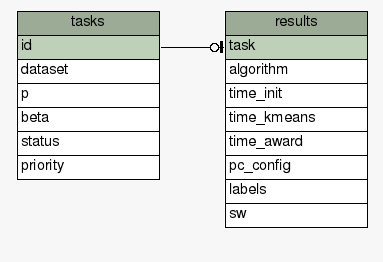
\includegraphics[scale=0.8]{img/relationships.png} 
			\end{center}
			\caption{Схема базы данных}
			\label{fig:relationships}
		\end{figure}
		
		В базе данных имеется всего две таблицы: \texttt{tasks} и \texttt{results}. Каждая запись таблицы \texttt{tasks} соответствует не более чем одной записи в \texttt{results}. Соответствие задается при помощи внешнего ключа \texttt{results.task}, который указывает на соответствующий идентификатор \texttt{tasks.id}. 
		
		Таблица \texttt{tasks} выполняет функцию синхронизацию по разделению заданий между потоками. Она заполняется заранее, до запуска изучаемых алгоритмов. Запись в этой таблице соответствует элементарному эксперименту с заданными значениями параметров, записанных в \texttt{tasks.p} и \texttt{tasks.beta}. Поле \texttt{tasks.dataset} определяет с каким из 330 файлов данных следует провести эксперимент, а вспомогательное поле  \texttt{tasks.priority} позволяет изменять порядок выполнения заданий. Особое внимание заслуживает столбец \texttt{tasks.status}, благодаря которому исключается одновременное выполнение несколькими потоками одного и того же задания. Изначально статус задачи выставлен \texttt{NULL}. Если поток приступает к выполнению некоторого задания, то этот поток выставляет статус задачи \texttt{'PEND'}. Таким образом, все остальные потоки не могут взять на обработку это задание. Как только выполнение очередного задания закончено, поток выставляет соответствующую метку \texttt{'COMP'}. В той же транзакции происходит запись результата в таблицу \texttt{results}.
		
		Результат представленный в таблице \texttt{results} хранит время, затраченное на выполнение каждого из этапов алгоритма $ A-Ward_{p\beta} $, значение характеристики SW а также некоторую вспомогательную информацию.
	
	\section{Результаты}
		Как было сказано выше, для вычисленных $ 1681 $ значений характеристики SW выбирается единственная пара параметров $ p^*, \beta^*  $, которые признаются оптимальными для каждого из рассматриваемых массивов данных. Рассматриваются две возможные стратегии выбора: (1) минимизирующая расстояние до начала координат и (2) минимизирующая расстояние до усреднённого максимума. После выбора $ p^*, \beta^*  $ производится выполнение алгоритма $ A-Ward_{p\beta} $ и для полученного разбиения вычисляется значение индекса ARI. Эти значения приведены в таблицах \ref{tab:ari-strategy1-sw} и \ref{tab:ari-strategy2-sw} соответственно для стратегий 1 и 2. В ячейках таблиц крупным шрифтом набраны средние значения по всем 10 массивам данных, а мелким шрифтом --- стандартные отклонения.
	
		\begin{table}[h!]
			\centering
			\caption{Значения индекса ARI для стратегии выбора 1 (оценка по SW) } \label{tab:ari-strategy1-sw}
			\begin{tabularx}{\textwidth}{|L{0.4\textwidth}|C{0.09\textwidth}|C{0.09\textwidth}|C{0.09\textwidth}|C{0.09\textwidth}|Z|}
				\hline
				dataset                           & 1-1000                      & 1-100                       &  1-200                      & 5-100                       & 5-200 \\ \hline
				kovaleva\_1000x15\_c7\_m100\_a0.5 & $ \underset{0.000}{1.000} $ & $ \underset{0.079}{0.894} $ & $ \underset{0.075}{0.897} $ & $ \underset{0.074}{0.920} $ & $ \underset{0.092}{0.903} $ \\ \hline
				kovaleva\_1000x15\_c12\_m60\_a0.5 & $ \underset{0.044}{0.977} $ & $ \underset{0.165}{0.749} $ & $ \underset{0.151}{0.781} $ & $ \underset{0.133}{0.755} $ & $ \underset{0.134}{0.838} $ \\ \hline
				kovaleva\_1000x15\_c19\_m35\_a0.5 & $ \underset{0.050}{0.821} $ & $ \underset{0.113}{0.605} $ & $ \underset{0.141}{0.602} $ & $ \underset{0.112}{0.608} $ & $ \underset{0.128}{0.626} $ \\ \hline
			\end{tabularx}
		\end{table}

		\begin{table}[h!]
			\centering
			\caption{Значения индекса ARI для стратегии выбора 2 (оценка по SW) } \label{tab:ari-strategy2-sw}
			\begin{tabularx}{\textwidth}{|L{0.4\textwidth}|C{0.09\textwidth}|C{0.09\textwidth}|C{0.09\textwidth}|C{0.09\textwidth}|Z|}
				\hline
				dataset                           & 1-1000                      & 1-100                       &  1-200                      & 5-100                       & 5-200 \\ \hline
				kovaleva\_1000x15\_c7\_m100\_a0.5 & $ \underset{0.000}{1.000} $ & $ \underset{0.042}{0.986} $ & $ \underset{0.052}{0.974} $ & $ \underset{0.062}{0.949} $ & $ \underset{0.062}{0.949} $ \\ \hline
				kovaleva\_1000x15\_c12\_m60\_a0.5 & $ \underset{0.044}{0.977} $ & $ \underset{0.218}{0.774} $ & $ \underset{0.183}{0.820} $ & $ \underset{0.173}{0.803} $ & $ \underset{0.186}{0.803} $ \\ \hline
				kovaleva\_1000x15\_c19\_m35\_a0.5 & $ \underset{0.050}{0.821} $ & $ \underset{0.079}{0.622} $ & $ \underset{0.115}{0.587} $ & $ \underset{0.088}{0.600} $ & $ \underset{0.127}{0.596} $ \\ \hline
			\end{tabularx}
		\end{table}

		Отдельный интерес представляет оценка допустимости использования характеристики $ SW  $ в практических приложениях. Для проведения такой оценки можно сравнить полученные экспериментальные результаты из таблиц \ref{tab:ari-strategy1-sw} и \ref{tab:ari-strategy2-sw} с результатами, в которых для выбора наилучшего значения $ p^*, \beta^*  $ использовался индекс ARI. Так как все массивы данных сгенерированы программно, то для этих данных известно истинное разбиение, с помощью которого и производится вычисление индекса $ ARI $. В таблицах  \ref{tab:ari-strategy1-ari}, \ref{tab:ari-strategy2-ari} приведены результаты подбора наилучших параметров алгоритма для случая если известно истинное разбиение.

		\begin{table}[h!]
			\centering
			\caption{Значения индекса ARI для стратегии выбора 1 (оценка по ARI)} \label{tab:ari-strategy1-ari}
			\begin{tabularx}{\textwidth}{|L{0.4\textwidth}|C{0.09\textwidth}|C{0.09\textwidth}|C{0.09\textwidth}|C{0.09\textwidth}|Z|}
				\hline
				dataset                           & 1-1000                      & 1-100                       &  1-200                      & 5-100                       & 5-200 \\ \hline
				kovaleva\_1000x15\_c7\_m100\_a0.5 & $ \underset{0.000}{1.000} $ & $ \underset{0.079}{0.894} $ & $ \underset{0.075}{0.897} $ & $ \underset{0.074}{0.920} $ & $ \underset{0.092}{0.903} $ \\ \hline
				kovaleva\_1000x15\_c12\_m60\_a0.5 & $ \underset{0.039}{0.978} $ & $ \underset{0.165}{0.749} $ & $ \underset{0.151}{0.781} $ & $ \underset{0.152}{0.790} $ & $ \underset{0.120}{0.850} $ \\ \hline
				kovaleva\_1000x15\_c19\_m35\_a0.5 & $ \underset{0.046}{0.829} $ & $ \underset{0.124}{0.625} $ & $ \underset{0.128}{0.609} $ & $ \underset{0.087}{0.580} $ & $ \underset{0.117}{0.611} $ \\ \hline
			\end{tabularx}
		\end{table}
		
		\begin{table}[h!]
			\centering
			\caption{Значения индекса ARI для стратегии выбора 2 (оценка по ARI)} \label{tab:ari-strategy2-ari}
			\begin{tabularx}{\textwidth}{|L{0.4\textwidth}|C{0.09\textwidth}|C{0.09\textwidth}|C{0.09\textwidth}|C{0.09\textwidth}|Z|}
				\hline
				dataset                           & 1-1000                      & 1-100                       &  1-200                      & 5-100                       & 5-200 \\ \hline
				kovaleva\_1000x15\_c7\_m100\_a0.5 & $ \underset{0.000}{1.000} $ & $ \underset{0.042}{0.986} $ & $ \underset{0.052}{0.974} $ & $ \underset{0.062}{0.949} $ & $ \underset{0.062}{0.949} $ \\ \hline
				kovaleva\_1000x15\_c12\_m60\_a0.5 & $ \underset{0.039}{0.978} $ & $ \underset{0.221}{0.792} $ & $ \underset{0.183}{0.820} $ & $ \underset{0.192}{0.807} $ & $ \underset{0.188}{0.788} $ \\ \hline
				kovaleva\_1000x15\_c19\_m35\_a0.5 & $ \underset{0.046}{0.829} $ & $ \underset{0.088}{0.636} $ & $ \underset{0.108}{0.631} $ & $ \underset{0.090}{0.591} $ & $ \underset{0.100}{0.612} $ \\ \hline
			\end{tabularx}
		\end{table}

		Также для оценки применимости SW можно провести сравнительный анализ тепловых карт, изображенных на рисунках \ref{fig:sw} и \ref{fig:ari}. На этих картах по осям откладываются значения параметров $ p, \beta $, а цвет характеризует значение индекса. Чем ярче цвет, тем ближе это значение к 1, и наоборот --- тёмный цвет соответствует отрицательным значениям.

		Так как цель работы состоит в поиске подхода, который позволил бы сократить время вычислений, то требуется также проанализировать время работы для всех предложенных вариантов. В таблице \ref{tab:times} приведены времена (в секундах) вычислений для всех рассматриваемых алгоритмов и стандартные отклонения (мелким шрифтом).
		\begin{table}[h!]
			\centering
			\caption{Время вычислений (сек.)} \label{tab:times}
			\begin{tabularx}{\textwidth}{|L{0.4\textwidth}|C{0.09\textwidth}|C{0.09\textwidth}|C{0.09\textwidth}|C{0.09\textwidth}|Z|}
				\hline
				dataset                           & 1-1000                      & 1-100                       &  1-200                      & 5-100                       & 5-200 \\ \hline
				kovaleva\_1000x15\_c7\_m100\_a0.5 & $  \underset{1158}{5651} $ & $ \underset{109}{805}  $ & $ \underset{186}{1270} $ & $ \underset{371}{4093} $ & $ \underset{799}{6256} $ \\ \hline
				kovaleva\_1000x15\_c12\_m60\_a0.5 & $   \underset{692}{9021} $ & $ \underset{53}{1215}  $ & $ \underset{147}{1855} $ & $ \underset{504}{6104} $ & $ \underset{581}{9328} $ \\ \hline
				kovaleva\_1000x15\_c19\_m35\_a0.5 & $ \underset{1261}{11413} $ & $ \underset{173}{1702} $ & $ \underset{231}{2686} $ & $ \underset{399}{8200} $ & $ \underset{806}{13376} $ \\ \hline
			\end{tabularx}
		\end{table}
		


	\begin{figure*}[t!]
		\centering
		\begin{subfigure}[t]{1\textwidth}
			\centering
			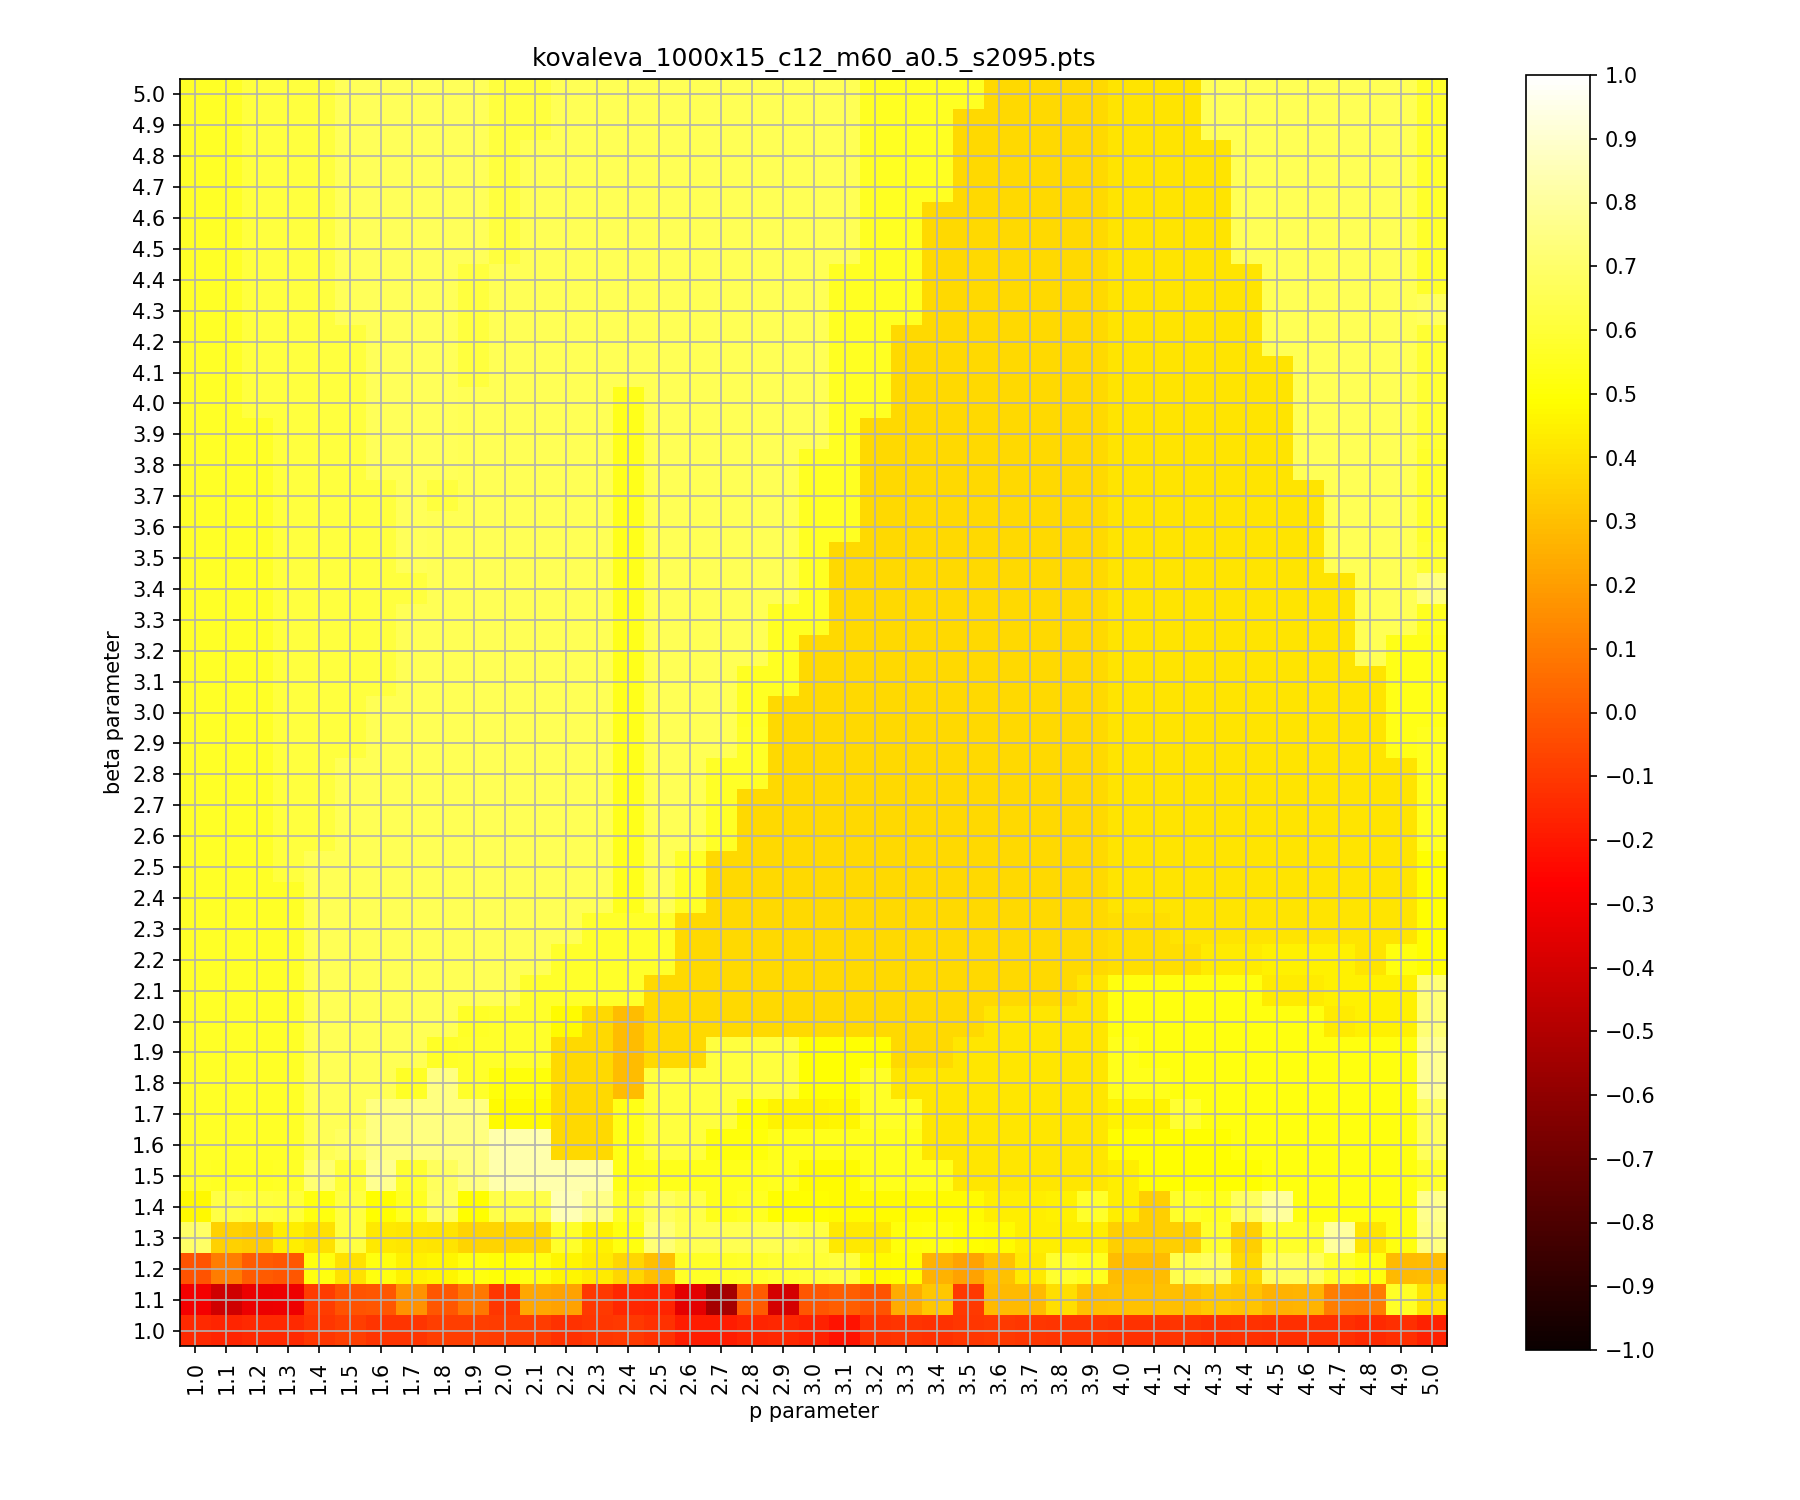
\includegraphics[width=1\linewidth, trim=1.4cm 1cm 2cm 0.5cm, clip]{img/sw/12/kovaleva_1000x15_c12_m60_a0.5_s2095/kovaleva_1000x15_c12_m60_a0.5_s2095.png}
			\caption{Полный набор данных}
			\label{fig:sw-1000}
		\end{subfigure}%
		~ 	
		
		\begin{subfigure}[t]{0.5\textwidth}
			\centering
			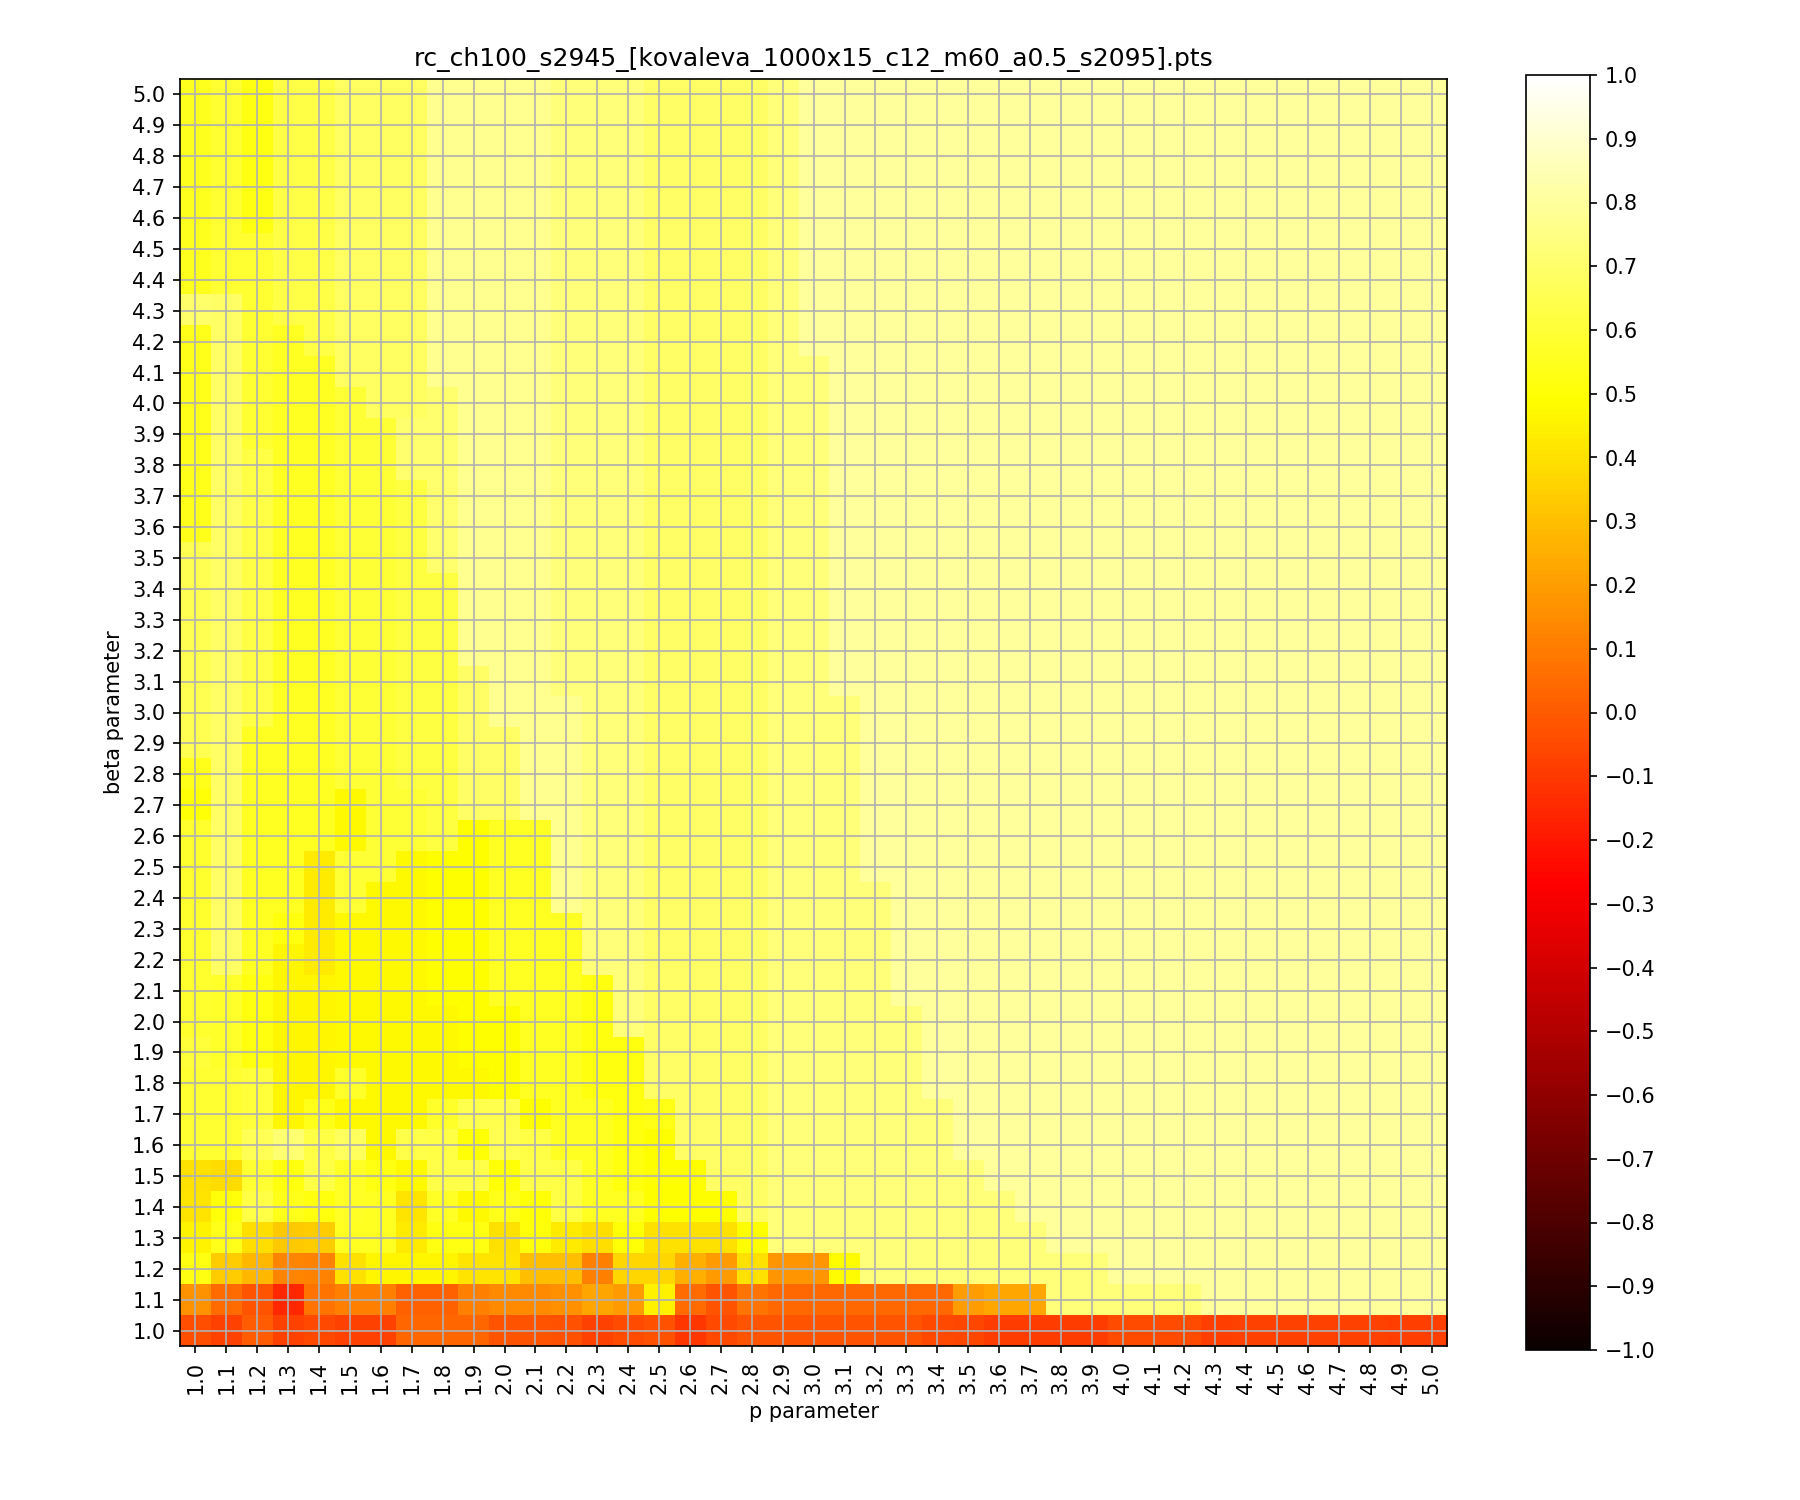
\includegraphics[width=1\linewidth, trim=1.4cm 1cm 2cm 0.5cm, clip]{img/sw/12/kovaleva_1000x15_c12_m60_a0.5_s2095/100/rc_ch100_s2945_[kovaleva_1000x15_c12_m60_a0.5_s2095].png}
			\caption{Оценка по выборке из 100 точек} \label{fig:sw-100}
		\end{subfigure}%
		~
		\begin{subfigure}[t]{0.5\textwidth}
			\centering
			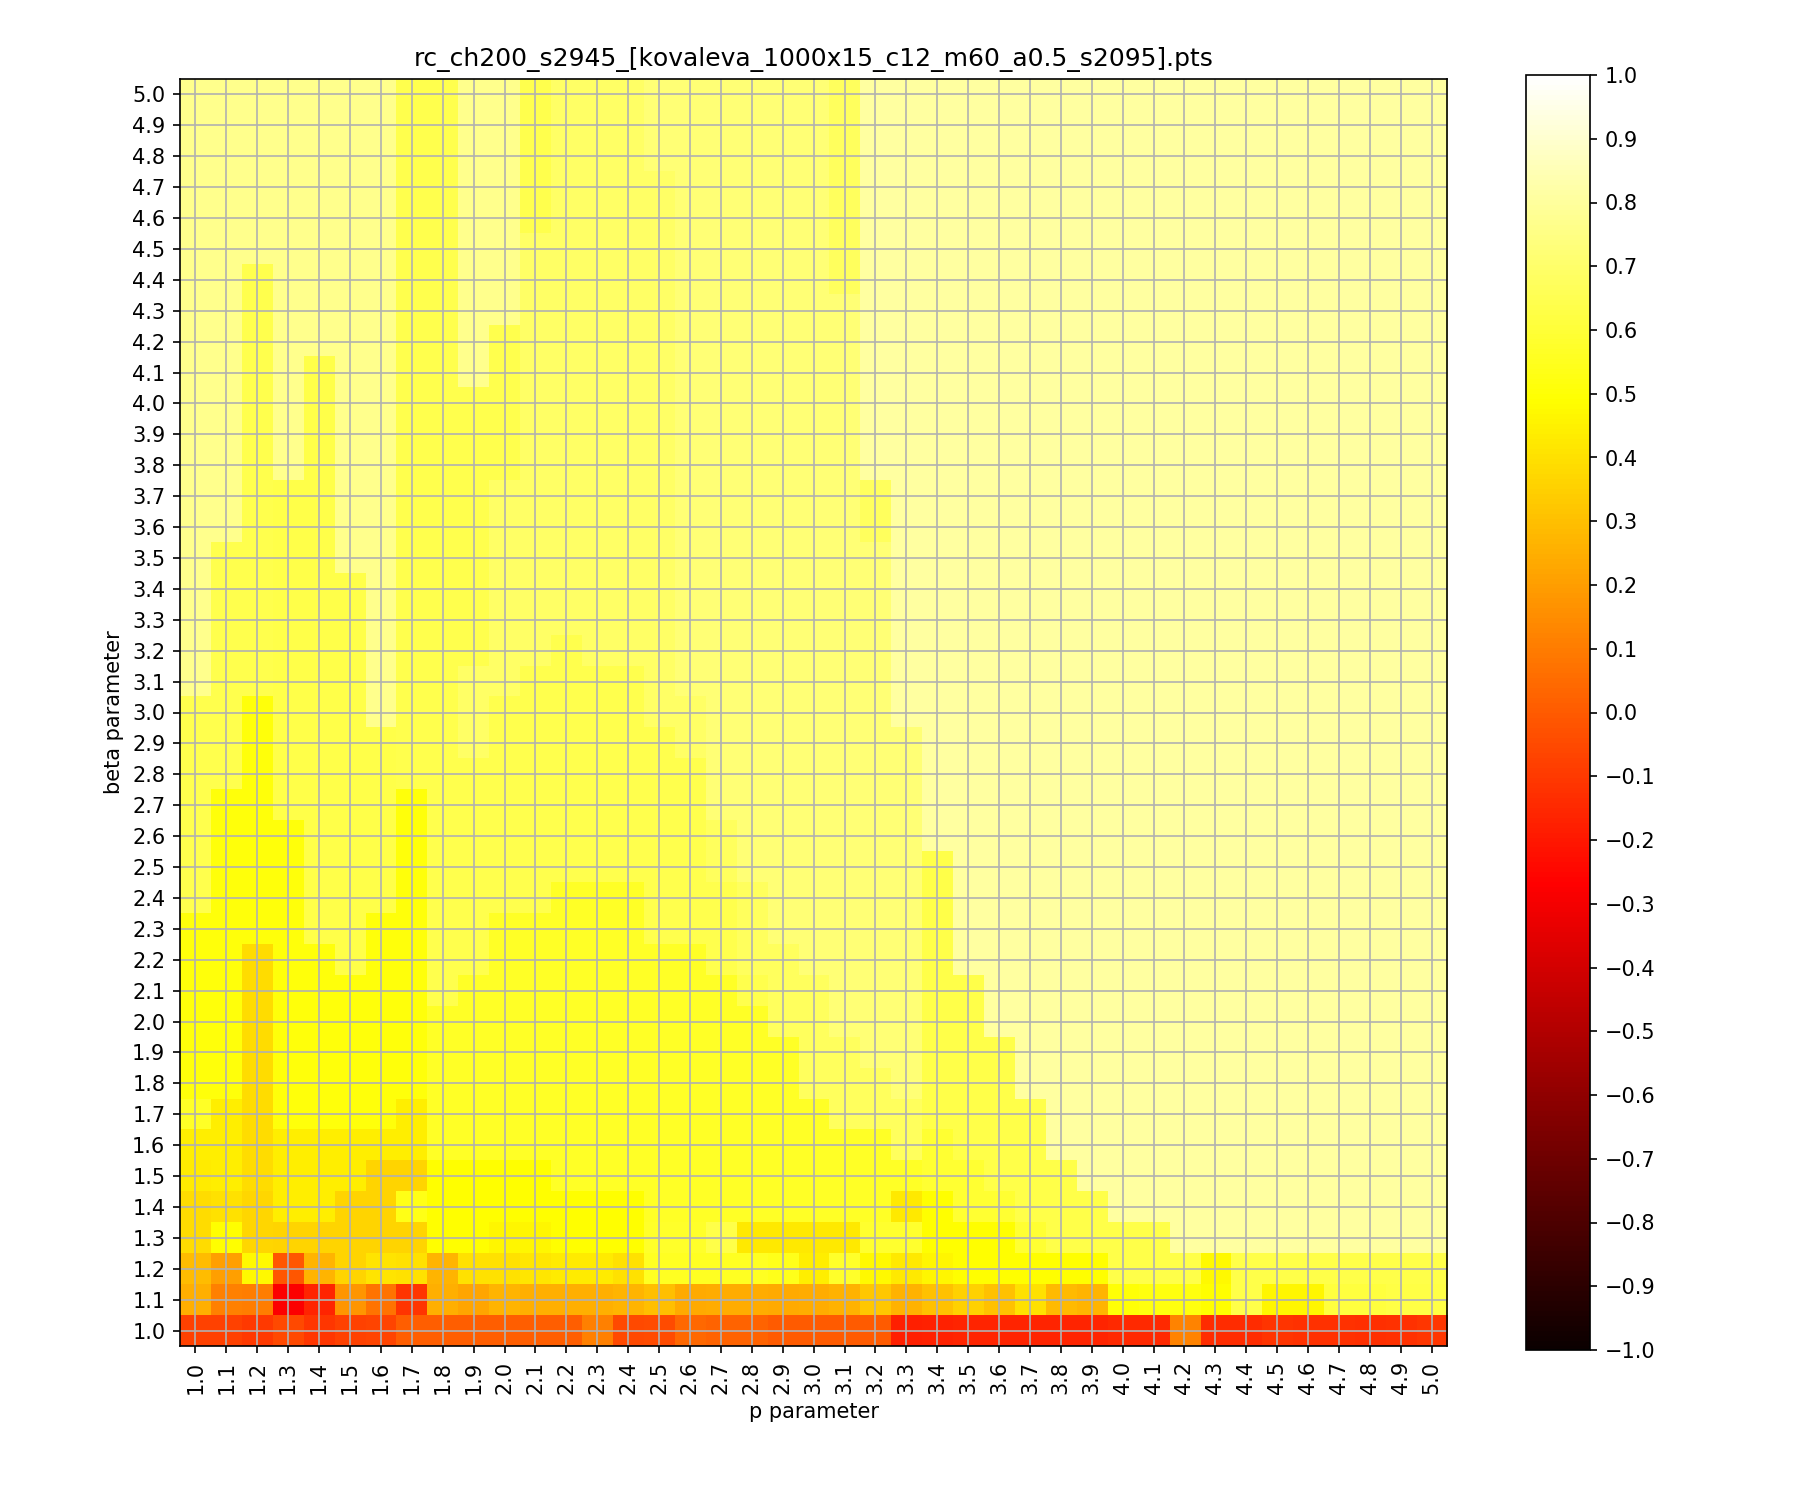
\includegraphics[width=1\linewidth, trim=1.4cm 1cm 2cm 0.5cm, clip]{img/sw/12/kovaleva_1000x15_c12_m60_a0.5_s2095/200/rc_ch200_s2945_[kovaleva_1000x15_c12_m60_a0.5_s2095].png}
			\caption{Оценка по выборке из 200 точек} \label{fig:sw-200}
		\end{subfigure}
		\caption{Значения характеристики SW} \label{fig:sw}
	\end{figure*}
	
	
	\newpage
	\begin{figure*}[t!]
		\centering
		\begin{subfigure}[t]{1\textwidth}
			\centering
			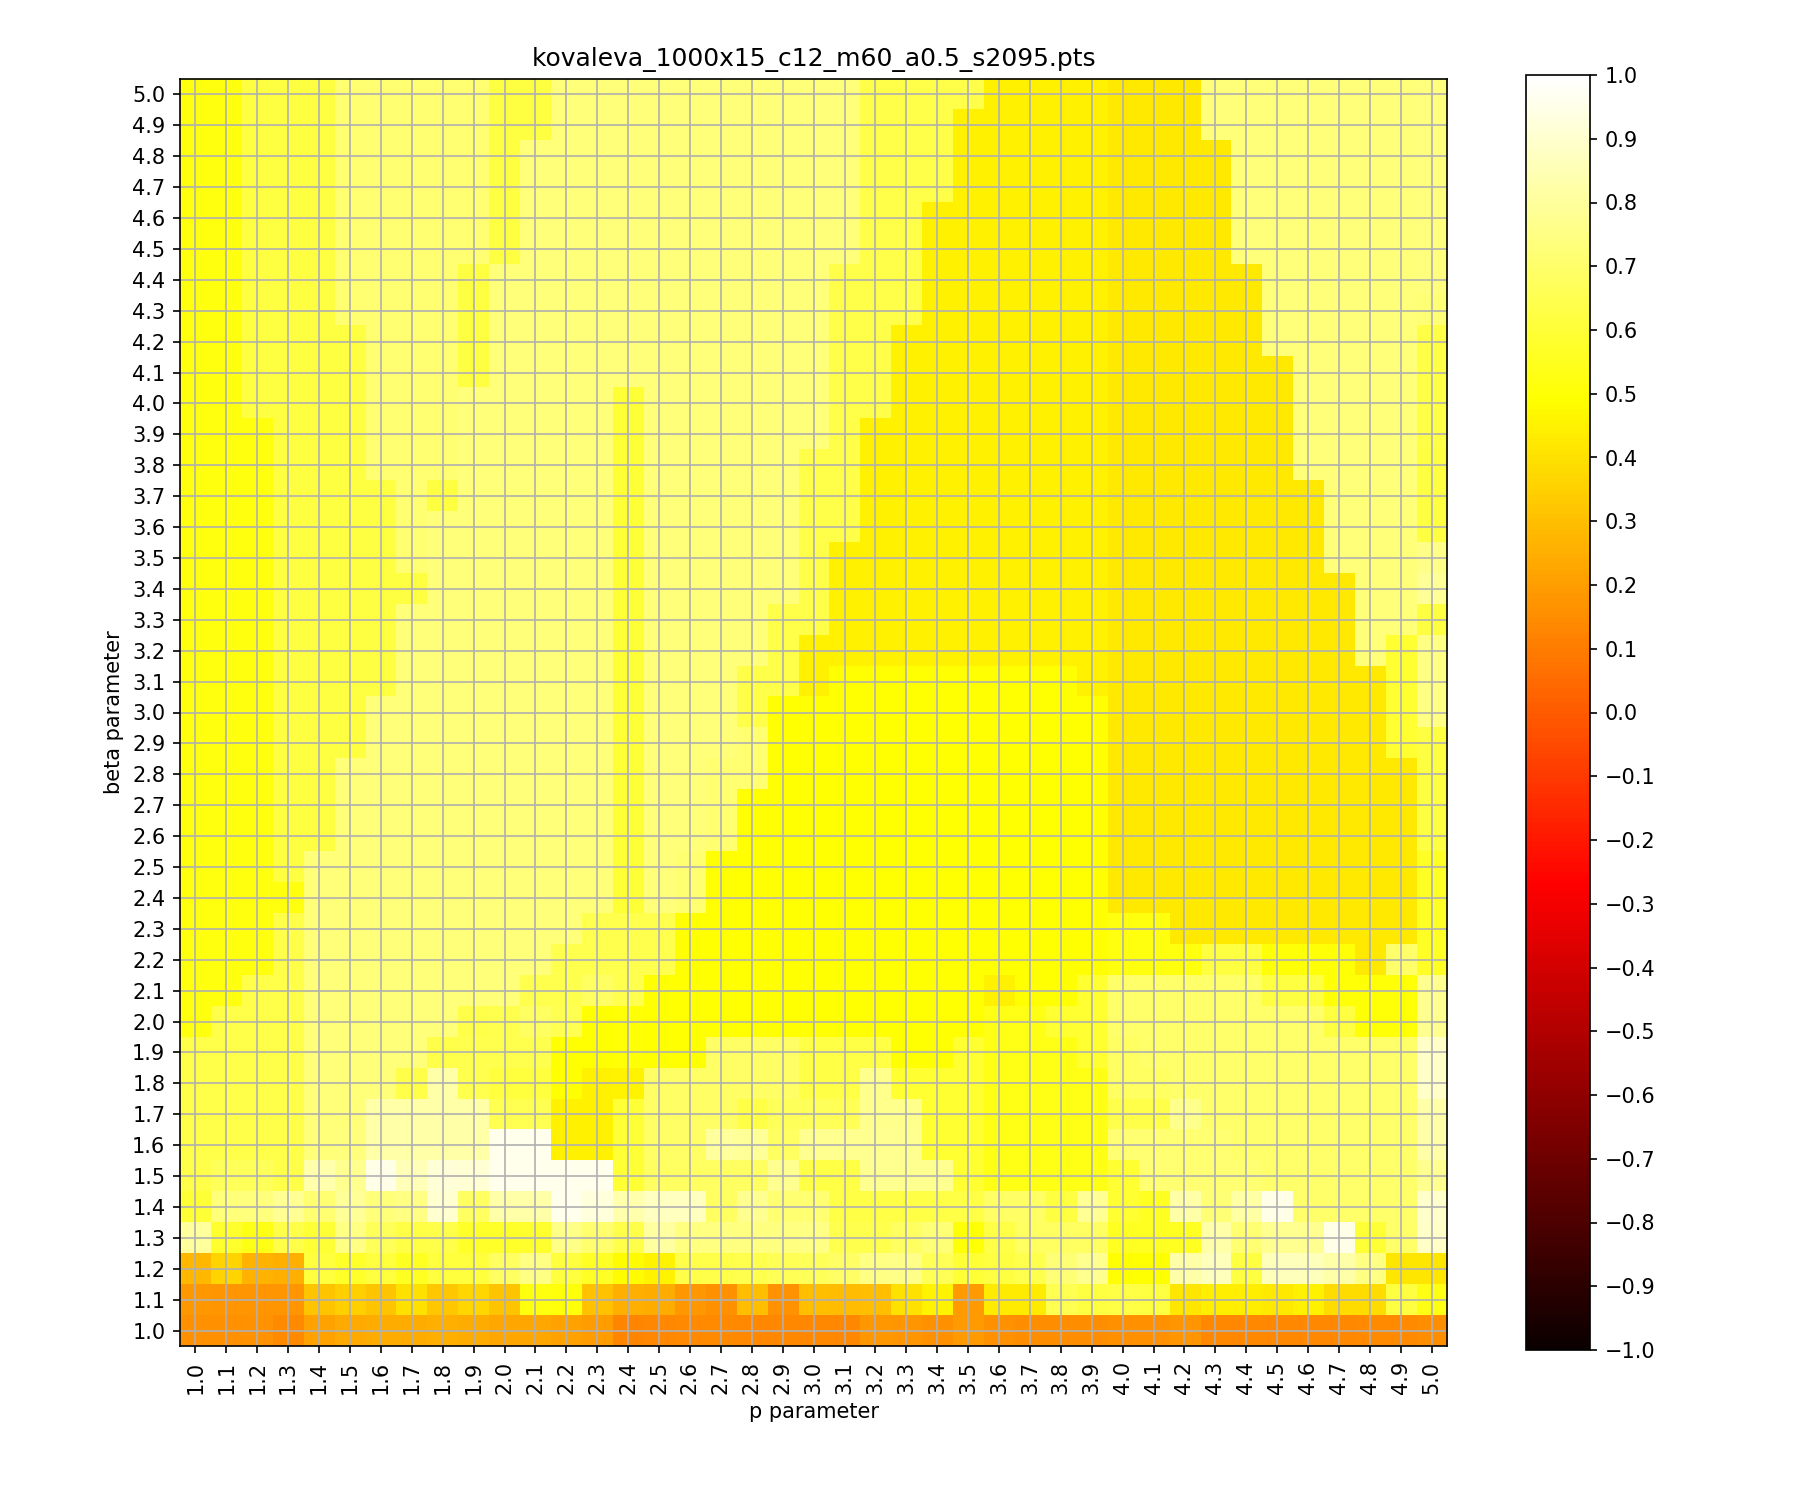
\includegraphics[width=1\linewidth, trim=1.4cm 1cm 2cm 0.5cm, clip]{img/ari/12/kovaleva_1000x15_c12_m60_a0.5_s2095/kovaleva_1000x15_c12_m60_a0.5_s2095.png}
			\caption{Полный набор данных}
			\label{fig:ari-1000}
		\end{subfigure}%
		~ 	
		
		\begin{subfigure}[t]{0.5\textwidth}
			\centering
			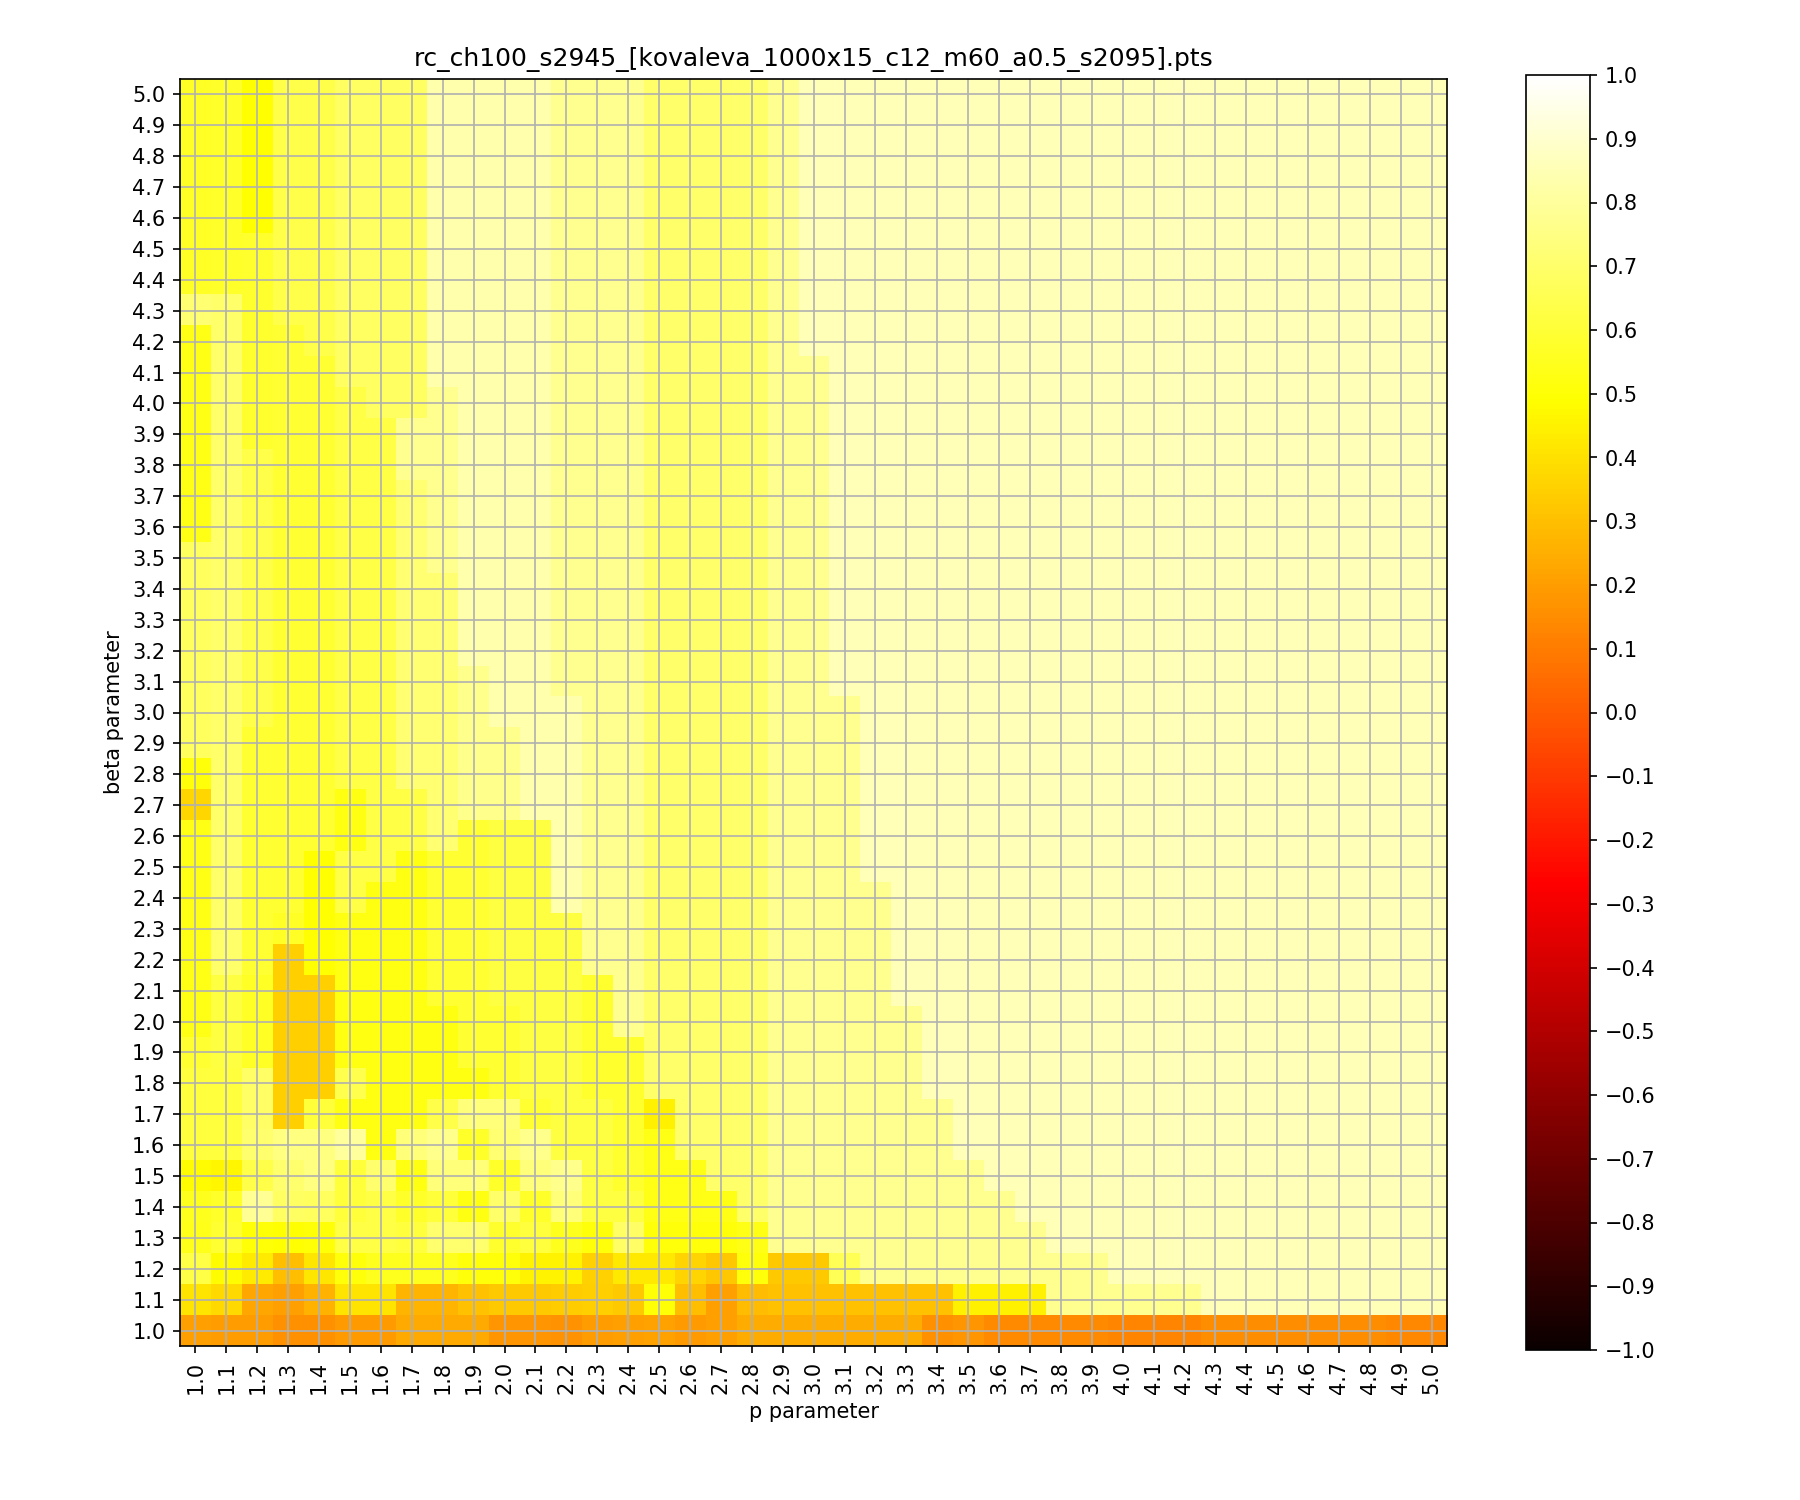
\includegraphics[width=1\linewidth, trim=1.4cm 1cm 2cm 0.5cm, clip]{img/ari/12/kovaleva_1000x15_c12_m60_a0.5_s2095/100/rc_ch100_s2945_[kovaleva_1000x15_c12_m60_a0.5_s2095].png}
			\caption{Оценка по выборке из 100 точек} \label{fig:ari-100}
		\end{subfigure}%
		~
		\begin{subfigure}[t]{0.5\textwidth}
			\centering
			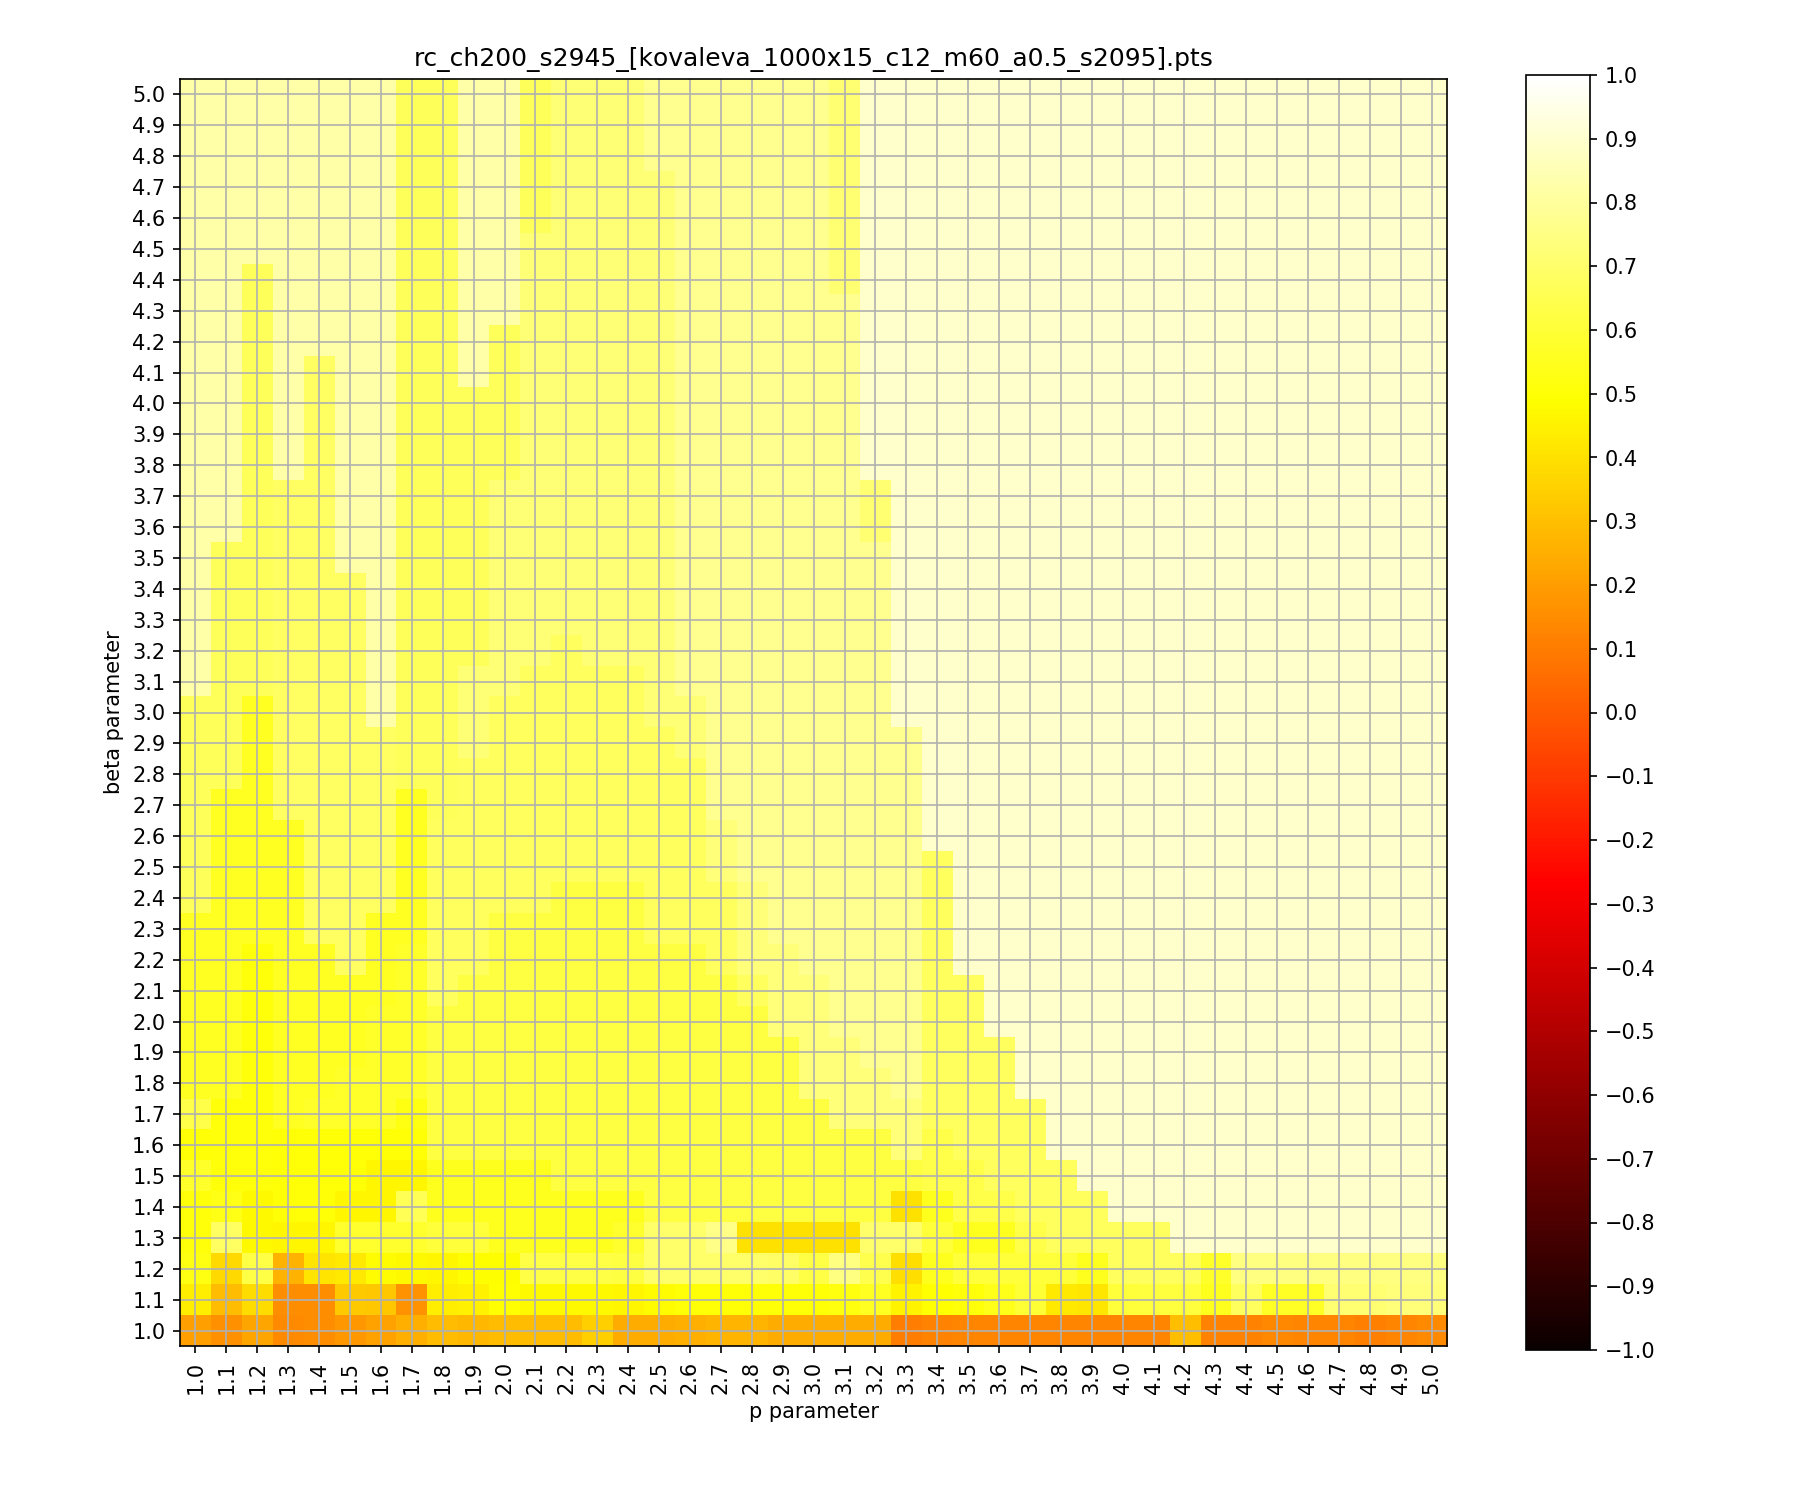
\includegraphics[width=1\linewidth, trim=1.4cm 1cm 2cm 0.5cm, clip]{img/ari/12/kovaleva_1000x15_c12_m60_a0.5_s2095/200/rc_ch200_s2945_[kovaleva_1000x15_c12_m60_a0.5_s2095].png}
			\caption{Оценка по выборке из 200 точек} \label{fig:ari-200}
		\end{subfigure}
		\caption{Значения индекса ARI} \label{fig:ari}
	\end{figure*}
			
	
	\section{Выводы}
		Таблицы \ref{tab:ari-strategy1-sw}, \ref{tab:ari-strategy2-sw} показывают, что стратегия выбора максимума 	\textnumero 2 имеет преимущество перед стратегией 	\textnumero 1 при применении однокаратной выборки (алгоритмы 1-100 и 1-200), а для пятикратной выборки результат второй стратегии несколько хуже. 
		
		Сравнительный анализ таблиц для оценки наилучших параметров по индексам ARI и SW  подтверждает правомерность использования эмпирической характеристики. К тому же выводу можно прийти при анализе тепловых карт: текстура изображения на рисунке \ref{fig:ari} практически полностью повторяется на рисунке \ref{fig:sw}, соответствующем характеристике SW.
		
		Целесообразность применения рассматриваемых подходов ограничена временем вычислений. Например, среднее время вычисления для пятикратной выборки по 200 объектов составляет 13376 секунд, что больше чем время полного перебора. 
		
		Таким образом, имеет смысл применять алгоритмы 1-100 и 1-200 для данных с небольшим количеством кластеров. Пятикратная выборка не оправдывает себя и не может быть применена ввиду ограничений по времени.
		
	
	
	% Список литературы
	\newpage
	% \nocite{anomalous} \nocite{ward} \nocite{boley} \nocite{tasoulis} \nocite{kovaleva} \nocite{mirkin}
	\addcontentsline{toc}{section}{Список литературы}
	\bibliography{bibliography}
	
	

\end{document}